\chapter{Implementation Details}
\label{chap:impl_details}

This chapter provides details about the implementation of the approach proposed in \Cref{chap:approach}. The implementation is written in Python 3. Its source code can be found in \Cref{attachment:sources}.

\section{Overview}

The implementation consists of three main components: a description processor, a scene composer, and a renderer. These components are depicted in \Cref{fig:impl_diagram}. The components and transitions between the components correspond to the drawing generation pipeline presented in \Cref{chap:approach}.
\begin{figure}[h]
    \centering
    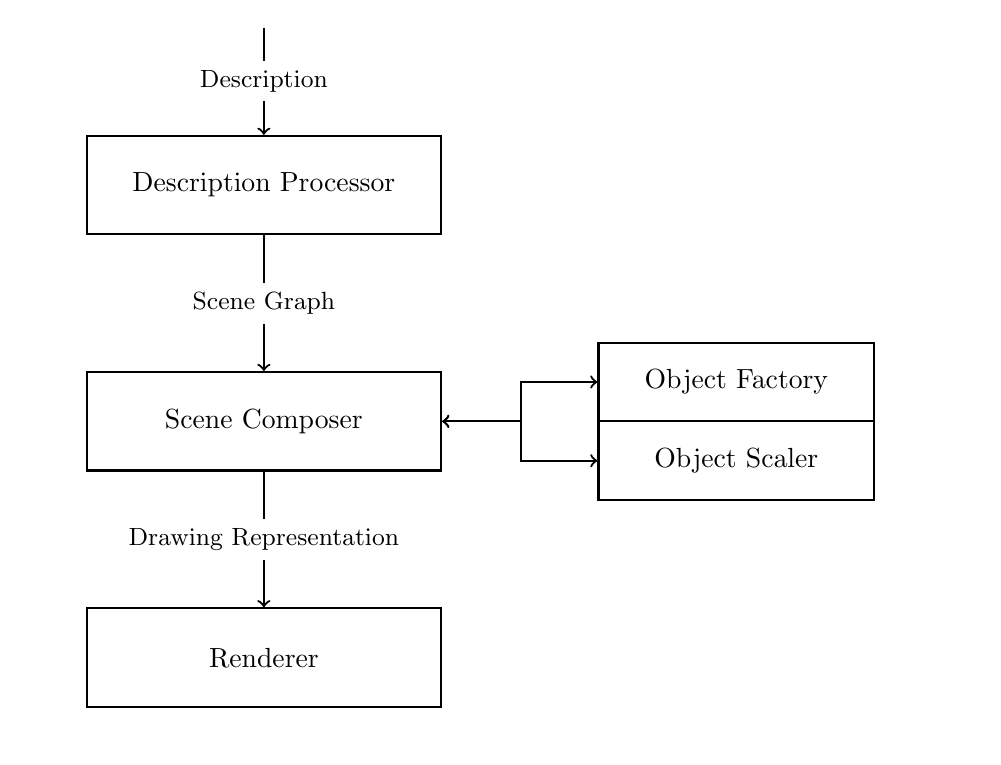
\begin{tikzpicture}[node distance=3cm]
        \tikzstyle{box} = [draw, thick, rectangle, minimum height=1.25cm, minimum width=4.5cm];
        \tikzstyle{smallerbox} = [draw, thick, rectangle, minimum height=1cm, minimum width=3.5cm];
    
        \clip (-3cm,-1cm) rectangle + (12cm,-9cm);

        \node(empty){};
        \node(descproc)[box, below of=empty]{Description Processor};
        \node(scenecomp)[box, below of=descproc]{Scene Composer};
        \node(renderer)[box, below of=scenecomp]{Renderer};

        \node(objfactory)[smallerbox, right of=scenecomp, yshift=0.5cm, xshift=3cm]{Object Factory};
        \node(objscaler)[smallerbox, right of=scenecomp, yshift=-0.5cm, xshift=3cm]{Object Scaler};

        \draw [->, thick] ++(0, -1cm) -- node[draw, fill=white, draw=none]{\small Description} (descproc);
        \draw [->, thick] (descproc) -- node[draw, fill=white, draw=none]{\small Scene Graph} (scenecomp);
        \draw [->, thick] (scenecomp) -- node[draw, fill=white, draw=none]{\small Drawing Representation} (renderer);
        \draw [<->, thick] (scenecomp.east) -- ++(1cm, 0) |- (objfactory);
        \draw [<->, thick] (scenecomp.east) -- ++(1cm, 0) |- (objscaler);
    \end{tikzpicture}
    \caption[Implementation diagram]{Implementation diagram.}
    \label{fig:impl_diagram}
\end{figure}

Besides the three main components, the diagram in \Cref{fig:impl_diagram} also contains two other components: an object factory and an object scaler. Together with the scene composer component, these two components implement the algorithms proposed in \fullref{sec:composing_scene}. Each of the components is discussed in more detail in the following sections.

\section{Description Processor}

The description processor is a component responsible for converting the input text into a scene graph. Description processor has one public method \verb|process|. The method has the following Python signature: 
\begin{verbatim}
process(self, text: str) -> Scene
\end{verbatim}

\Cref{attachment:sources} contains one implementation of the description processor - \break \verb|UDPipeDescriptionProcessor|. This implementation uses UDPipe \citep{straka2018udpipe} for syntactic analysis. The dependency tree traversal algorithm was described in the \fullref{sec:description_processing}. The \verb|resources/predicates| file contains a list of allowed predicates which can be processed by the processor.

\medskip

The \verb|Scene| class represents a scene graph. It contains two types of entities: \verb|Object| and \verb|Group| entities (subclasses of \verb|Entity|). Each entity has a list of relations represented by \verb|Relation|. 

\medskip

The \verb|Group| entity is just a convenience class which encapsulates other entities. Every group's relation is redirected to each entity within the group. We can extend the notation introduced in \fullref{sec:scene_graph_notation}, such that $[a, b]$ will denote a group of objects $a$ and $b$. Then $[a, b] \xrightarrow{p} c$ will effectively become $a \xrightarrow{p} c$ and $b \xrightarrow{p} c$. Similarly $a \xrightarrow{p} [b, c]$ will become $a \xrightarrow{p} c$ and $a \xrightarrow{p} c$.

\medskip

Apart from the relations, the \verb|Object| class also contains the attribute \verb|word|. This attribute holds a noun that describes the object. Note that in the case of composite nouns, this attribute may contain multiple words. 

\section{Scene Composer}

The scene composer determines the position of every object in the scene. The scene composer is a class with the following method:
\begin{verbatim}
compose(self, scene: Scene) -> List[PhysicalObject]
\end{verbatim}

\medskip

\verb|ConstraintComposer| is an implementation of the algorithm described in \fullref{sec:constraints}. The \verb|ConstraintComposer| associates each object in the scene with a corresponding \verb|Constraint| object. Then it uses these constraints to determine the positions using the described Monte Carlo algorithm. 

\medskip

The \verb|Constraint| is an abstract callable class. As opposed to the constraint function defined in \fullref{sec:constraints}, the \verb|Constraint| object operates on a batch of coordinates. It returns a Boolean array that masks the coordinates which satisfy the constraint. Using the notation from Section \ref{sec:scene_graph_notation}, we can describe the Python \verb|Constraint| call method:
\begin{verbatim}
__call__(self, xs: np.ndarray, ys: np.ndarray) -> np.ndarray
\end{verbatim}
As a mapping between two vectors:
\begin{align}
[(x_0, y_0), \ldots, (x_n, y_n)] \mapsto [C_{a,b}^p(x_0, y_0), \ldots, C_{a,b}^p(x_n, y_n)]
\end{align}

The scene composer generates a single set of random coordinates for one object. These coordinates are applied to every constraint associated with the object. The resulting boolean arrays are summed as integer arrays. By applying $argmax$ to this array, we find an index of coordinates that satisfy most of the constraints. These coordinates are used as the object's position. In other words, for a fixed object $a$, we set its position to be $(x_i, y_i)$, where:
\begin{align}
i = \argmax \sum_{(b, p)} [C_{a,b}^p(x_0, y_0), \ldots, C_{a,b}^p(x_n, y_n)]
\end{align}

\subsection{Constraints}
\label{sec:constraints_impl}

\Cref{sec:rule_based_constraints} lists a set of elementary constraints. In this section, we take a closer look at these constraints, describe how they are implemented and how they are combined to define constraints for specific adpositions. All constraints are implemented as subclasses of \verb|Constraint| which was described in the previous section. The constraints are initialised with an object and predicate that relates to the object. Information about the object and predicate are used to determine whether a point in plane satisfies the constraint.

\medskip

The \verb|OnConstraint| takes the upper $25\%$ of the object's drawing strokes. The constraint tests if a point is within a certain distance from these strokes. The distance is specified by attribute \verb|limit|.

\medskip

The \verb|SideConstraint| defines a half-plane. All points in this half-plane satisfy the constraint.  The constraint has two attributes -- \verb|direction| and \verb|offset|. The \verb|direction| attribute is a vector normal to the half-plane boundary.  The \verb|offset| attribute moves the boundary further away from the object.

\medskip

The \verb|BoxConstraint| is satisfied whenever a point lies inside a bounding box of the object to which the constraint relates. In addition, the implementation also contains an attribute \verb|scale| that can scale the bounding box up or down.

\medskip

The \verb|InsideConstraint| tests whether a point lies within an area spanned by the object it relates to. The area is given by strokes of drawing associated with the object. We consider each stroke to be a polygon. We test whether a point lies inside a polygon defined by one of the strokes. Some strokes contain many line segments, which could lead to a slow evaluation of the constraint. Hence, we apply the Ramer-Douglas-Peucker \citep{douglas1973algorithms} algorithm to the drawing to reduce its number of line segments.

\medskip

The primary purpose of \verb|DisjunctionConstraint| is to combine other non-overlapping constraints. The constraint is satisfied when any of the constraints it encapsulates is satisfied. Since we assume the encapsulated constraints are non-overlapping, only one of the constraints can be satisfied at a time. The same could be achieved by specifying more constraints for a single predicate. However, using the disjunction constraint does not require evaluating all the constraints~-- the evaluation ends after the first satisfied constraint. The non-overlapping regions can be seen in the right image of \Cref{fig:monte_carlo:1}. 

\medskip

\Cref{tab:rule_based_constraints_impl} below shows how the elementary constraints are used in the rule-based approach to form constraint functions for adpositions listed in \Cref{sec:rule_based_constraints}.

\begin{table}[ht]
    \small
    \centering
    \begin{threeparttable}
        \begin{tabular}{p{0.2\linewidth}|p{0.7\linewidth}}
            \textbf{Adposition} & \textbf{Elementary constraint} \\
            \hline \hline
            \emph{in}        &  \verb|InsideConstraint()| \\
            \hline
            \emph{inside}    & \verb|InsideConstraint()| \\
            \hline
            \emph{inside of} & \verb|InsideConstraint()| \\
            \hline
            \emph{on}        & \verb|OnConstraint()| \\
            \hline
            \emph{under}    & \verb|SideConstraint(direction=(0, 1))| \\
            \hline
            \emph{below}    & \verb|SideConstraint(direction=(0, 1))| \\
            \hline
            \emph{above}     & \verb|SideConstraint(direction=(0, -1))| \\
            \hline
            \emph{behind}    & \verb|BoxConstraint()| \\
            \hline
            \emph{in front of} & \verb|BoxConstraint()| \\
            \hline
            \emph{next to} & \begin{minipage}[t]{\linewidth}
            \begin{verbatim}
DisjunctionConstraint([
    SideConstraint(direction=(-1, 0)),
    SideConstraint(direction=(1, 0))
])\end{verbatim}
            \end{minipage}\vspace{4pt} \\
            \hline
            unknown & \begin{minipage}[t]{\linewidth}
            \begin{verbatim}
DisjunctionConstraint([
    SideConstraint(direction=(-1, 0)),
    SideConstraint(direction=(1, 0)),
    SideConstraint(direction=(0, 1)),
    SideConstraint(direction=(0, -1)),
])\end{verbatim}
            \end{minipage}\vspace{4pt}
        \end{tabular}
        \begin{tablenotes}
            \small
            \item Some constructor arguments are omitted for brevity.
        \end{tablenotes}
    \end{threeparttable}
    \caption[Rule-based constraints implementation]{Rule-based constraints implementation.}
    \label{tab:rule_based_constraints_impl}
\end{table}

\verb|ClassifierConstraint| implements the classfier-based approach described in \fullref{sec:classifier_based_constraints}. The classifier uses \emph{scikit-learn's} \citep{scikit-learn} multi-layered perceptron classifier trained on the \emph{Scene Graph} dataset. The trained model is loaded from \verb|resources/sklearn/constraints.model| file. All relevant details about the model are discussed in \Cref{sec:classifier_based_constraints}.

\subsection{Object Factory}

The object factory is a class with a method with the following Python signature:
\begin{verbatim}
get_physical_object(self, obj: Object) -> PhysicalObject
\end{verbatim}

\verb|QuickDrawObjectFactory| instantiates a \verb|PhysicalObject| using Quick, Draw! \citep{quickdraw} Data. It uses a \verb|WordEmbedding| class for resolving objects which are not present in the \emph{Quick, Draw!} categories.

\medskip

\verb|WordEmbedding| class is a wrapper around a \emph{fasttext}  \citep{bojanowski2017enriching} model. It has a single method \verb|most_similar_word(self, word: 'str') -> 'str'| which finds the most similar word from a list of words based on the cosine similarity. The list of words is, in this case, a list of \emph{Quick, Draw!} categories.

\subsection{Object Scaler}

The object scaler determines the object sizes. The object scaler class has the following Python signature:

\begin{verbatim}
scale(self, sub: PhysicalObject, obj: PhysicalObject, 
            pred: str) -> float
\end{verbatim}

This method scales the subject \verb|sub|. The size estimation may use the context given by the object \verb|obj| or the predicate \verb|pred|. The size estimation strategy depends on the implementation. We provide two object scaler implementations~--~\verb|AbsoluteObjectScaler| and \verb|RelativeObjectScaler|. These clases implement the object scaling methods described in \fullref{sec:determining_obj_size}.

\medskip

The \verb|AbsoluteObjectScaler| scales the \verb|sub| object according to a table of absolute (hand crafted) sizes located in \verb|resources/quickdraw/attributes.csv|. The file contains a width and/or height for the given \emph{Quick, Draw!} category.

\medskip

The \verb|RelativeObjectScaler| takes into account both subject and object (\verb|sub| and \verb|obj|). The subject is scaled according to a table of relative sizes located in \verb|resources/quickdraw/attributes_relative.csv| file. The file contains width and height ratios for the given pair of \emph{Quick, Draw!} categories. The size of \verb|obj| has to be known before calling the \verb|scale| method. Its size is multiplied by the ratio specified in the file to determine the subject's size.

\section{Renderer}

The renderer is the last component in the system. The only purpose of the renderer is to render a final drawing from a \verb|PhysicalObject| list. Two different renderers are provided. The first one, \verb|SimpleRenderer|, renders a PNG image. This renderer is used in the command-line interface. The other renderer has a form of a web application written in JavaScript. The composed scene served over HTTP is rendered onto an HTML canvas. The web interface is discussed in more detail in \fullref{sec:web_interface}.
